\chapter{Einführung in Model-Based Systems Engineering}

\begin{lernziele}
Nach diesem Kapitel verstehen Sie den Unterschied zwischen dokumentenzentrierter Entwicklung und modellbasierter Entwicklung. Sie können erklären, warum ein zentrales Modell bei komplexen Projekten nützlich ist.
\end{lernziele}

\section{Dokumentenzentrierte Entwicklung}
In vielen Projekten liegen Informationen verstreut vor: Anforderungen in Excel, Architektur in PowerPoint, Schnittstellen in Word, Aufgaben in Jira und Code in Git. Das funktioniert eine Zeit lang, wird aber unübersichtlich. Sobald Änderungen auftreten, ist unklar, welche Dokumente angepasst werden müssen.

\section{Modellbasierte Entwicklung}
\gls{mbse} verwendet ein Modell als zentrale Informationsquelle. Dieses Modell enthält Anforderungen, Struktur, Verhalten, Schnittstellen und Tests. Das Modell ersetzt nicht den Code und nicht jede technische Spezifikation. Es verbindet aber die wichtigsten Informationen.

\section{Vorteile von MBSE}
Die wichtigsten Vorteile sind Nachvollziehbarkeit, Konsistenz und bessere Kommunikation. Ein Entwickler sieht, welche Anforderung eine Komponente erfüllt. Ein Tester sieht, welcher Test zu welcher Anforderung gehört. Ein Projektleiter erkennt, welche Teile von einer Änderung betroffen sind.

\begin{hinweisbox}
MBSE bedeutet nicht, dass jedes Detail modelliert werden muss. Ein gutes Modell ist so detailliert wie nötig und so einfach wie möglich.
\end{hinweisbox}

\section{MBSE im Roboterprojekt}
Für unseren Roboter modellieren wir Anforderungen, Systemstruktur, Datenflüsse, Verhalten, ROS2-Komponenten und Tests. Damit entsteht eine Kette von der Idee bis zur Umsetzung.

\begin{center}
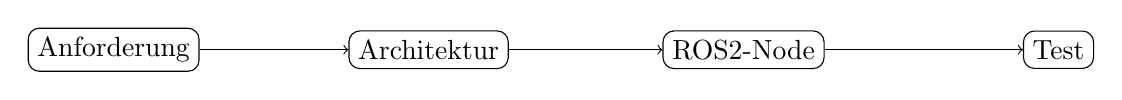
\begin{tikzpicture}[node distance=1.6cm]
\node (req) [draw, rounded corners] {Anforderung};
\node (arch) [draw, rounded corners, right of=req, xshift=2.4cm] {Architektur};
\node (impl) [draw, rounded corners, right of=arch, xshift=2.4cm] {ROS2-Node};
\node (test) [draw, rounded corners, right of=impl, xshift=2.4cm] {Test};
\draw[->] (req) -- (arch);
\draw[->] (arch) -- (impl);
\draw[->] (impl) -- (test);
\end{tikzpicture}
\end{center}

\section{Grenzen von MBSE}
MBSE löst keine schlechten technischen Entscheidungen. Ein Modell kann falsch, veraltet oder unnötig kompliziert sein. Der Nutzen entsteht nur, wenn das Modell gepflegt wird und echte Entscheidungen unterstützt.

\begin{uebungbox}
Erstellen Sie eine Tabelle mit drei Spalten: Information, klassischer Speicherort und Speicherort im MBSE-Modell. Tragen Sie Anforderungen, Schnittstellen, Tests und ROS2-Nodes ein.
\end{uebungbox}
